\documentclass[sigconf,authordraft]{acmart}
\usepackage{tikz}
\usetikzlibrary{arrows}

\newcommand{\den}[2][]{
\left\llbracket#2\right\rrbracket^{#1}
}
\newcommand{\low}[1]{
\left\lfloor#1\right\rfloor
}
\newcommand{\denml}[1]{
  \den[ml]{#1}
}
\newcommand{\denev}[1]{
  \den[ev]{#1}
}

\newcommand{\squash}{\itemsep=0pt\parskip=0pt}
\newcommand{\uavam}{\textsf{UAVAM}}
\newcommand{\useram}{\textsf{UserAM}}
\newcommand{\platam}{\textsf{PlatformAM}}
\newcommand{\selam}{\textsf{seL4AM}}
\newcommand{\uboot}{\textsf{UBOOT}}
\newcommand{\duhk}{\textsf{DUHK}}
\newcommand{\M}[1]{\ensuremath{M_{\mathsf{#1}}}}
\newcommand{\E}[1]{\ensuremath{E_{\mathsf{#1}}}}
\newcommand{\R}[1]{\ensuremath{R_{\mathsf{#1}}}}
\newcommand{\sign}[2]{\ensuremath{\{#1\}_{#2^{-1}}}}

%% The article template's documentation, available at
%% \url{https://www.acm.org/publications/proceedings-template}, has a
%% complete explanation of these commands and tips for their effective
%% use.

\setcopyright{acmcopyright}
\copyrightyear{2020}
\acmYear{2020}
\acmDOI{0000}

%% These commands are for a PROCEEDINGS abstract or paper.
\acmConference[Attestation Negotiation]{Working Paper on Attestation
  Negotiation}{20 January, 2020}{Lawrence, KS}
\acmBooktitle{No Book}
\acmPrice{0.00}
\acmISBN{0000}

%%\acmSubmissionID{123-A56-BU3}


\begin{document}

\title{Negotiating Attestation Protocols}

\author{Anna Fritz}
\email{arfritzz@ku.edu}
\author{Perry Alexander}
\orcid{0000-0002-5387-9157}
\email{palexand@ku.edu}
\affiliation{%
  \institution{ITTC - The University of Kansas}
  \streetaddress{2335 Irving Hill Rd}
  \city{Lawrence}
  \state{Kansas}
  \country{USA}
  \postcode{66045}
}

\renewcommand{\shortauthors}{Fritz and Alexander}

\begin{abstract}
  Abstract goes here
\end{abstract}

%%
%% The code below is generated by the tool at http://dl.acm.org/ccs.cfm.
%% Please copy and paste the code instead of the example below.
%%
\begin{CCSXML}
<ccs2012>
 <concept>
  <concept_id>10010520.10010553.10010562</concept_id>
  <concept_desc>Computer systems organization~Embedded systems</concept_desc>
  <concept_significance>500</concept_significance>
 </concept>
 <concept>
  <concept_id>10010520.10010575.10010755</concept_id>
  <concept_desc>Computer systems organization~Redundancy</concept_desc>
  <concept_significance>300</concept_significance>
 </concept>
 <concept>
  <concept_id>10010520.10010553.10010554</concept_id>
  <concept_desc>Computer systems organization~Robotics</concept_desc>
  <concept_significance>100</concept_significance>
 </concept>
 <concept>
  <concept_id>10003033.10003083.10003095</concept_id>
  <concept_desc>Networks~Network reliability</concept_desc>
  <concept_significance>100</concept_significance>
 </concept>
</ccs2012>
\end{CCSXML}

\ccsdesc[500]{Computer systems organization~Embedded systems}
\ccsdesc[300]{Computer systems organization~Redundancy}
\ccsdesc{Computer systems organization~Robotics}
\ccsdesc[100]{Networks~Network reliability}

\keywords{TBD}

\maketitle

\section{Introduction}

Introduction goes here.

\begin{figure}[hbtp]
  \centering
  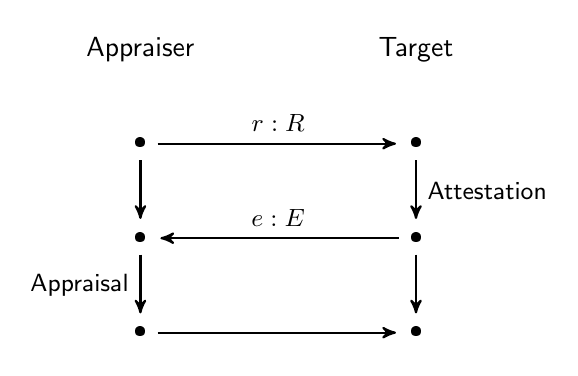
\begin{tikzpicture}[->,>=stealth',shorten >=1pt,auto,node distance=1.2cm,
  thick,main node/.style={rectangle,%fill=blue!20,draw,
    font=\sffamily,minimum height=2mm,minimum width=2mm},
  io node/.style={rectangle,
    font=\sffamily,minimum height=5mm,minimum width=10mm}]

  \node[main node] (APPTITLE) {Appraiser};
  \node[main node] (TARTITLE) [node distance=3.5cm, right of=APPTITLE] {Target};
  \node[main node] (SREQ) [below of=APPTITLE] {\textbullet};
  \node[main node] (RREQ) [below of=TARTITLE] {\textbullet};
  \node[main node] (REV) [below of=SREQ] {\textbullet};
  \node[main node] (SEV) [below of=RREQ] {\textbullet};
  \node[main node] (APP) [below of=REV] {\textbullet};
  \node[main node] (NONE) [below of=SEV] {\textbullet};
    
  \path[every node/.style={font=\sffamily\small, fill=white,inner sep=1pt}]
    (SREQ) edge node[above=1mm] {$r:R$} (RREQ)
    (SEV) edge node[above=1mm] {$e:E$} (REV)
    (APP) edge (NONE)
    (SREQ) edge (REV)
    (RREQ) edge node[right=1mm] {Attestation} (SEV)
    (SEV) edge (NONE)
    (REV) edge node[left=1mm] {Appraisal} (APP)
    ;
\end{tikzpicture}

%%% Local Variables: 
%%% mode: latex
%%% TeX-master: "negotiation20"
%%% End:

  \caption[Attestation architecture]{Remote attestation architecture
    showing an \emph{appraiser} making an attestation request of a
    \emph{target}.}
  \Description{Remote attestation basic architecture.}
  \label{fig:remote-attestation}
\end{figure}

\begin{figure}[hbtp]
  \centering
  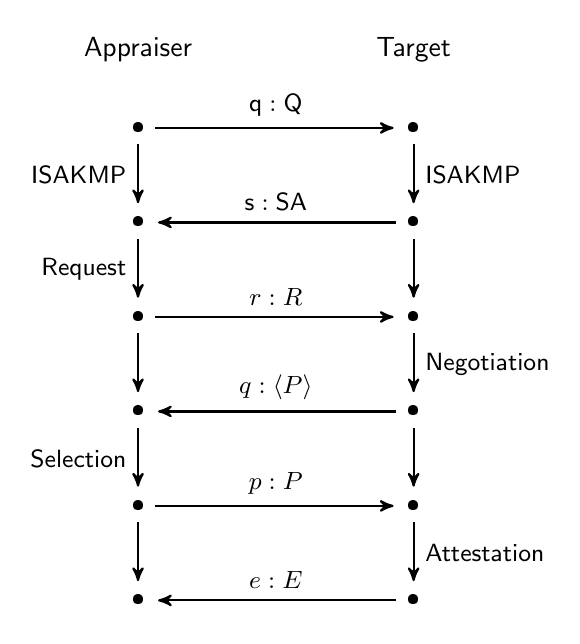
\begin{tikzpicture}[->,>=stealth',shorten >=1pt,auto,node distance=1.2cm,
  thick,main node/.style={rectangle,%%fill=blue!20,draw,
    font=\sffamily,minimum height=2mm,minimum width=2mm}]


  \node[main node] (RQ) {\textbullet};
  \node[main node] (SA) [below of=RQ] {\textbullet};
  \node[main node] (NM) [below of=SA] {\textbullet};
  \node[main node] (AM) [below of=NM] {\textbullet};
  \node[main node] (CP) [below of=AM] {\textbullet};
  \node[main node] (HW) [below of=CP] {\textbullet};
%%  \node[main node] (AP) [below of=HW] {\textbullet};
  \node[main node] (HWE) [node distance=3.5cm, right of=HW] {\textbullet};
  \node[main node] (CPE) [node distance=3.5cm, right of=CP] {\textbullet};
  \node[main node] (AME) [node distance=3.5cm, right of=AM] {\textbullet};
  \node[main node] (NME) [node distance=3.5cm, right of=NM] {\textbullet};
  \node[main node] (SAE) [node distance=3.5cm, right of=SA] {\textbullet};  
  \node[main node] (RQE) [node distance=3.5cm, right of=RQ] {\textbullet};  
  \node[main node] (IN) [node distance=1.0cm, above of=RQ] {Appraiser};
  \node[main node] (OUT) [node distance=1.0cm, above of=RQE] {Target};
    

  \path[every node/.style={font=\sffamily\small, fill=white,inner sep=1pt}]
    (RQ) edge node[above=1mm] {$\mathsf{q:Q}$} (RQE)
    (SAE) edge node[above=1mm] {$\mathsf{s:SA}$} (SA)
    (NM) edge node[above=1mm] {$r:R$} (NME)
    (AME) edge node[above=1mm] {$q:\langle P \rangle$} (AM)
    (CP) edge node[above=1mm] {$p:P$} (CPE)
    (HWE) edge node[above=1mm] {$e:E$} (HW)
    (RQ) edge node[left=1mm] {ISAKMP} (SA)
    (RQE) edge node[right=1mm] {ISAKMP} (SAE)
    (SA) edge node[left=1mm] {Request} (NM)
    (SAE) edge node[right=1mm] {} (NME)
    (NM) edge node[left=1mm] {} (AM)
    (NME) edge node[right=1mm] {Negotiation} (AME)
    (AM) edge node[left=1mm] {Selection} (CP)
    (AME) edge node[right=1mm] {} (CPE)
    (CP) edge node[left=1mm] {} (HW)
    (CPE) edge node[right=1mm] {Attestation} (HWE)
%%    (HW) edge node[left=1mm] {Appraisal} (AP)
    ;
\end{tikzpicture}

%%% Local Variables: 
%%% mode: latex
%%% TeX-master: "negotiation20"
%%% End:

  \caption[Attestation process]{Attestation process.}
  \Description{Attestation sequence.}
  \label{fig:sequence-fig}
\end{figure}

\begin{figure}[hbtp]
  \centering
  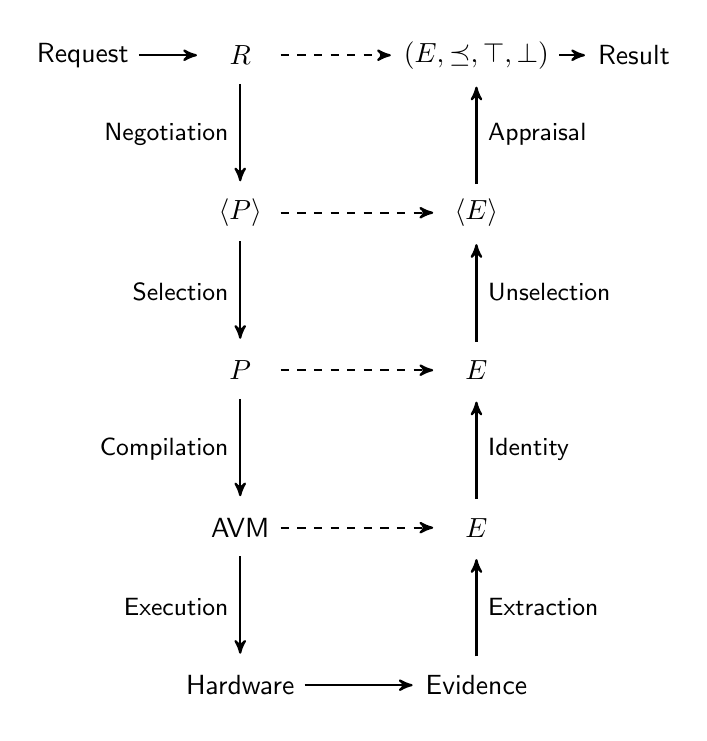
\begin{tikzpicture}[->,>=stealth',shorten >=1pt,auto,node distance=2.0cm,
  thick,main node/.style={rectangle,%%fill=blue!20,draw,
    font=\sffamily,minimum height=7mm,minimum width=10mm}]

  \node[main node] (Request) {$R$};
  \node[main node] (Proposal) [below of=Request] {$\langle P\rangle $};
  \node[main node] (Phrase) [below of=Proposal] {$P$};
  \node[main node] (AttInt) [below of=Phrase] {$\mathsf{AVM}$};
  \node[main node] (Hardware) [below of=AttInt] {Hardware};
  \node[main node] (Bits) [node distance=3.0cm, right of=Hardware] {Evidence};
  \node[main node] (VME) [node distance=3.0cm, right of=AttInt] {$E$};
  \node[main node] (Evidence) [node distance=3.0cm, right of=Phrase] {$E$};
  \node[main node] (EvidenceVec) [node distance=3.0cm, right of=Proposal] {$\langle E\rangle$};
  \node[main node] (Result) [node distance=3.0cm, right of=Request]
  {$(E,\preceq,\top,\bot)$};
  \node[main node] (IN) [node distance=2.0cm, left of=Request] {Request};
  \node[main node] (OUT) [node distance=2.0cm, right of=Result] {Result};
    

  \path[every node/.style={font=\sffamily\small, fill=white,inner sep=1pt}]
    (IN) edge (Request)
    (Request) edge node[left=1mm] {Negotiation} (Proposal)
    (Proposal) edge node[left=1mm] {Selection} (Phrase)
    (Phrase) edge node[left=1mm] {Compilation} (AttInt)
    (AttInt) edge node[left=1mm] {Execution} (Hardware)
    (Hardware) edge node[below=1mm] {} (Bits)
    (AttInt) edge [dashed] node[below=1mm] {} (VME)
    (Phrase) edge [dashed] node[below=1mm] {} (Evidence)
    (Proposal) edge [dashed] node[below=1mm] {} (EvidenceVec)
    (Request) edge [dashed] node[below=1mm] {} (Result)
    (Bits) edge node[right=1mm] {Extraction} (VME)
    (VME) edge node[right=1mm] {Identity} (Evidence)
    (Evidence) edge node[right=1mm] {Unselection} (EvidenceVec)
    (EvidenceVec) edge node[right=1mm] {Appraisal} (Result)
    (Result) edge (OUT)
    ;
\end{tikzpicture}

%%% Local Variables: 
%%% mode: latex
%%% TeX-master: "negotiation20"
%%% End:

  \caption[Attestation process]{Certification figure.}
  \Description{Certification figure.}
  \label{fig:certification-fig}
\end{figure}

\section{Conclusions}

Conclusions go here.

\bibliographystyle{ACM-Reference-Format}
\bibliography{sldg}

\end{document}

